% ************************************************************************
%
% Introduction
%
% ************************************************************************
\chpos{22mm}{10mm}

\chapter[Introduction]{Introduction}
\markboth{\thechapter\ \ Introduction}{\thechapter\ \ Introduction}
\label{ch1:introduction}

%\mysquote{0.8\textwidth}{Quote text.}{Author (\oldstylenums{1000} - \oldstylenums{1100})}

% ************************************************************************
% sources:
% https://www.quantamagazine.org/why-the-first-drawings-of-neurons-were-defaced-20170928/
% https://www.npr.org/sections/health-shots/2017/01/26/511455876/art-exhibition-celebrates-drawings-by-the-founder-of-modern-neuroscience
% https://www.nytimes.com/2018/01/18/arts/design/brain-neuroscience-santiago-ramon-y-cajal-grey-gallery.html
% https://www.brainpickings.org/2017/02/23/beautiful-brain-santiago-ramon-y-cajal/
\section{Neuron cell reconstruction} 
\lettrine{F}{ascination} with the neuron cells dates to the time when the glance into the sample of the silver-stained neuronal brain tissue over a century ago made it possible to gain insight into the intricate network that forms the very essence of the nervous system. The remarkable and groundbreaking drawings of Santiago Ram\'{o}n y Cajal \cite{swanson2017,ramon2008histologia}, neuroscience founding father, remain today as vivid as and fresh as the images captured by the latest fluorescence microscope, processed and rendered with the novel computer software. Ever since the discovery of the \textit{neuron doctrine}\footnote{Every neuron in the brain is separate. Neurons conduct information in a defined direction and communicate across the synapses.} \cite{glickstein2006golgi} and the early hand-made illustrations of the microscope-magnified samples of the brain tissue, numerous scientists and researchers of various backgrounds and interests have been trying to gain a deeper insight into the nervous system and the captivating mechanism of, arguably, one of the most complex and mysterious organs - brain. Numerous technical obstacles stand out when reaching out to such vastly unknown world, primarily due to the physical inaccessibility and the generally intangible nature of the whole system. Neuron cell thus represents a core building block of the brain and the nervous system. It appears in variety of shapes and specializations \cite{ascolitrees}. The estimated number of neuron cells in a human brain amounts to 89 billion \cite{herculano2009human} - number comparable to the count of stars in the Milky Way galaxy. Each neuron \textit{add: neuron dimensions} is further connected to 50 thousand other neurons on average which results in a very powerful computational network and an extremely efficient information storage. Captivating mechanism of the brain is an everlasting research topic as the complex functionality of the brain defines much of the activities, even the those such as consciousness. Discovering how the brain works is one of the grand unanswered questions of our era and central to diverse fields such as physics, mathematics, biology and recently prominent - computer science.

Nervous system activity is also manifested with the physical appearance of its neuron cells. Morphology of the single cell, shape of the neuronal network, topology or connectivity react to the external conditions or external stimuli. With the imaging tools such as fluorescence microscopy, the physical appearance the morphology of the single cell can be captured at micro meter scale can be inspected and recorded. Indeed, the studies that require deeper analysis make use of the imaging techniques that can reach nano meter scale, such as electron microscopy. In other words, accurate quantification of the cell shape is an important step towards better understanding of the cell functionality. Quantification of the neuronal structure is crucial in many neuroscience studies \cite{halavi2012digital} and quantification from microscopic images is identified as one of the major technical challenges in the digital era of neuroscience \cite{peng2015diadem}.

The advancements in informatics made it possible (Fig.~\ref{ch1__fig1}) to utilize computers to solve the neuroinformatics challenges over recent decades. With the ever growing amount of data, the processing of the information remains a challenge.   

\begin{figure}
	\begin{center}
		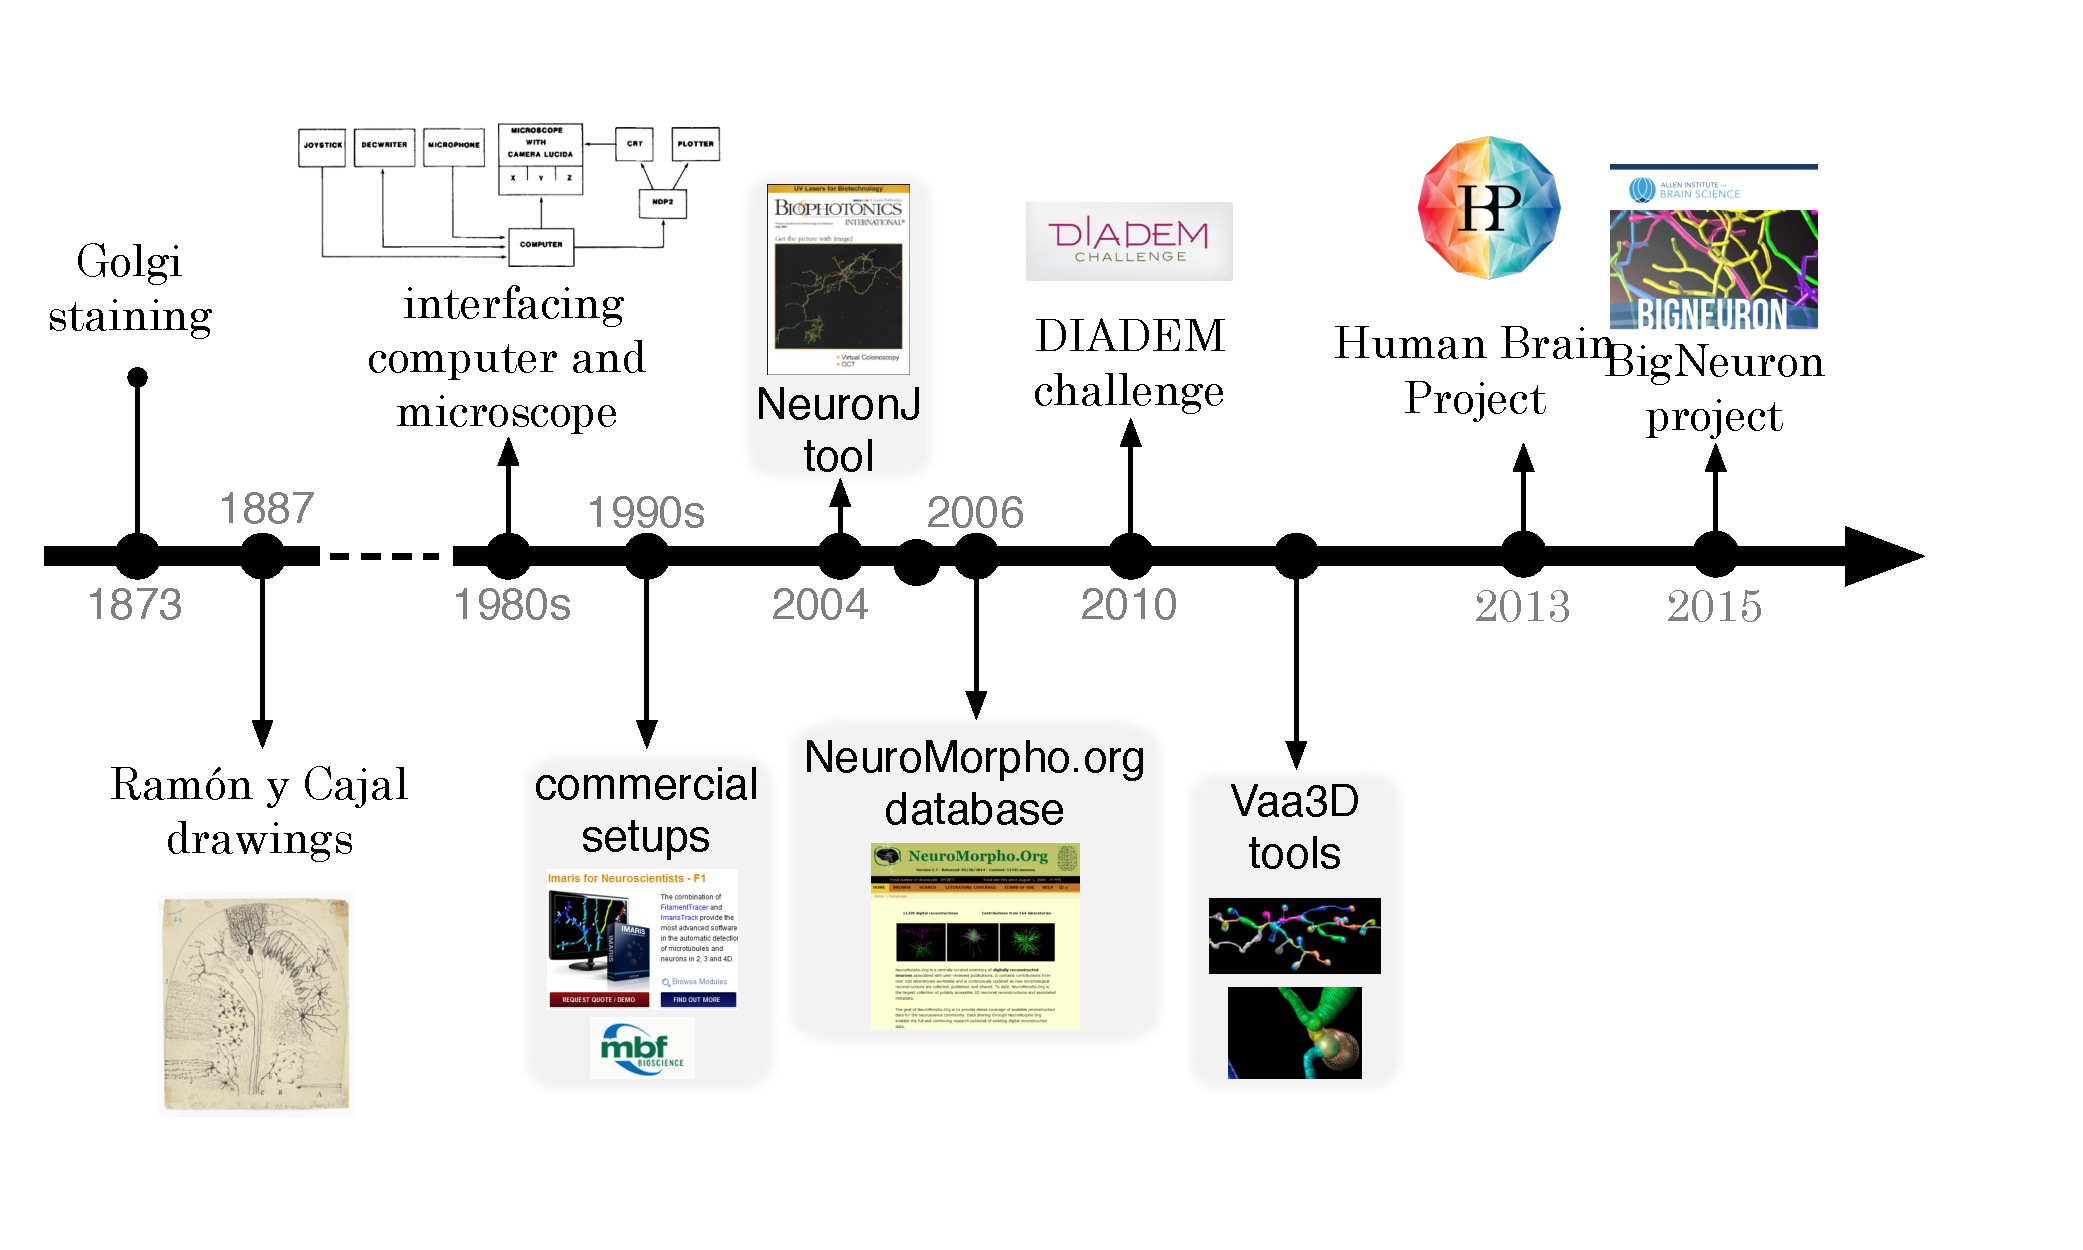
\includegraphics[width=\textwidth]{ch1_fig1}
	\end{center}
	\vspace{-3ex}
	\caption{Brief history of the neuron reconstruction. \textit{Corrections: Cajal drawings as separate item, and dating 1887-1892.}}
	\vspace{-1ex}
	\label{ch1__fig1}
\end{figure}

\section{Essential obstacles in neuron reconstruction}
The key obstacles concerning the full, accurate and robust automation of the neuron reconstruction \cite{meijering2010neuron,donohue2011automated,acciai2016automated} can be seen through the number of factors.

\textit{Morphology} the structural ambiguities of the diverse neuron cells (Fig.~\ref{}) often intractable to the human visual comprehension.

\textit{Noise} noisy image input (imaging on the boundary of the resolution limits in case of the light microscopy).

\textit{Data size} ever increasing size of the image volume needed to be correctly processed in reasonable time.

Aforementioned factors impose much of the computational barrier \cite{peng2011proof,svoboda2011past} in attempt to consistently produce human-comparable digital reconstructions. The real datasets, therefore, commonly leave with the persisting need for human expert assistance to obtain the optimal output. 

\section{Neuron tracing in fluorescence microscopy images}
%One of the key Java tools is the ImageJ library \cite{abramoff2004image}. 

\subsection{Extracting the correct tree}

\subsection{Bayesian methods in neuron tracing}

\begin{figure}
\begin{center}
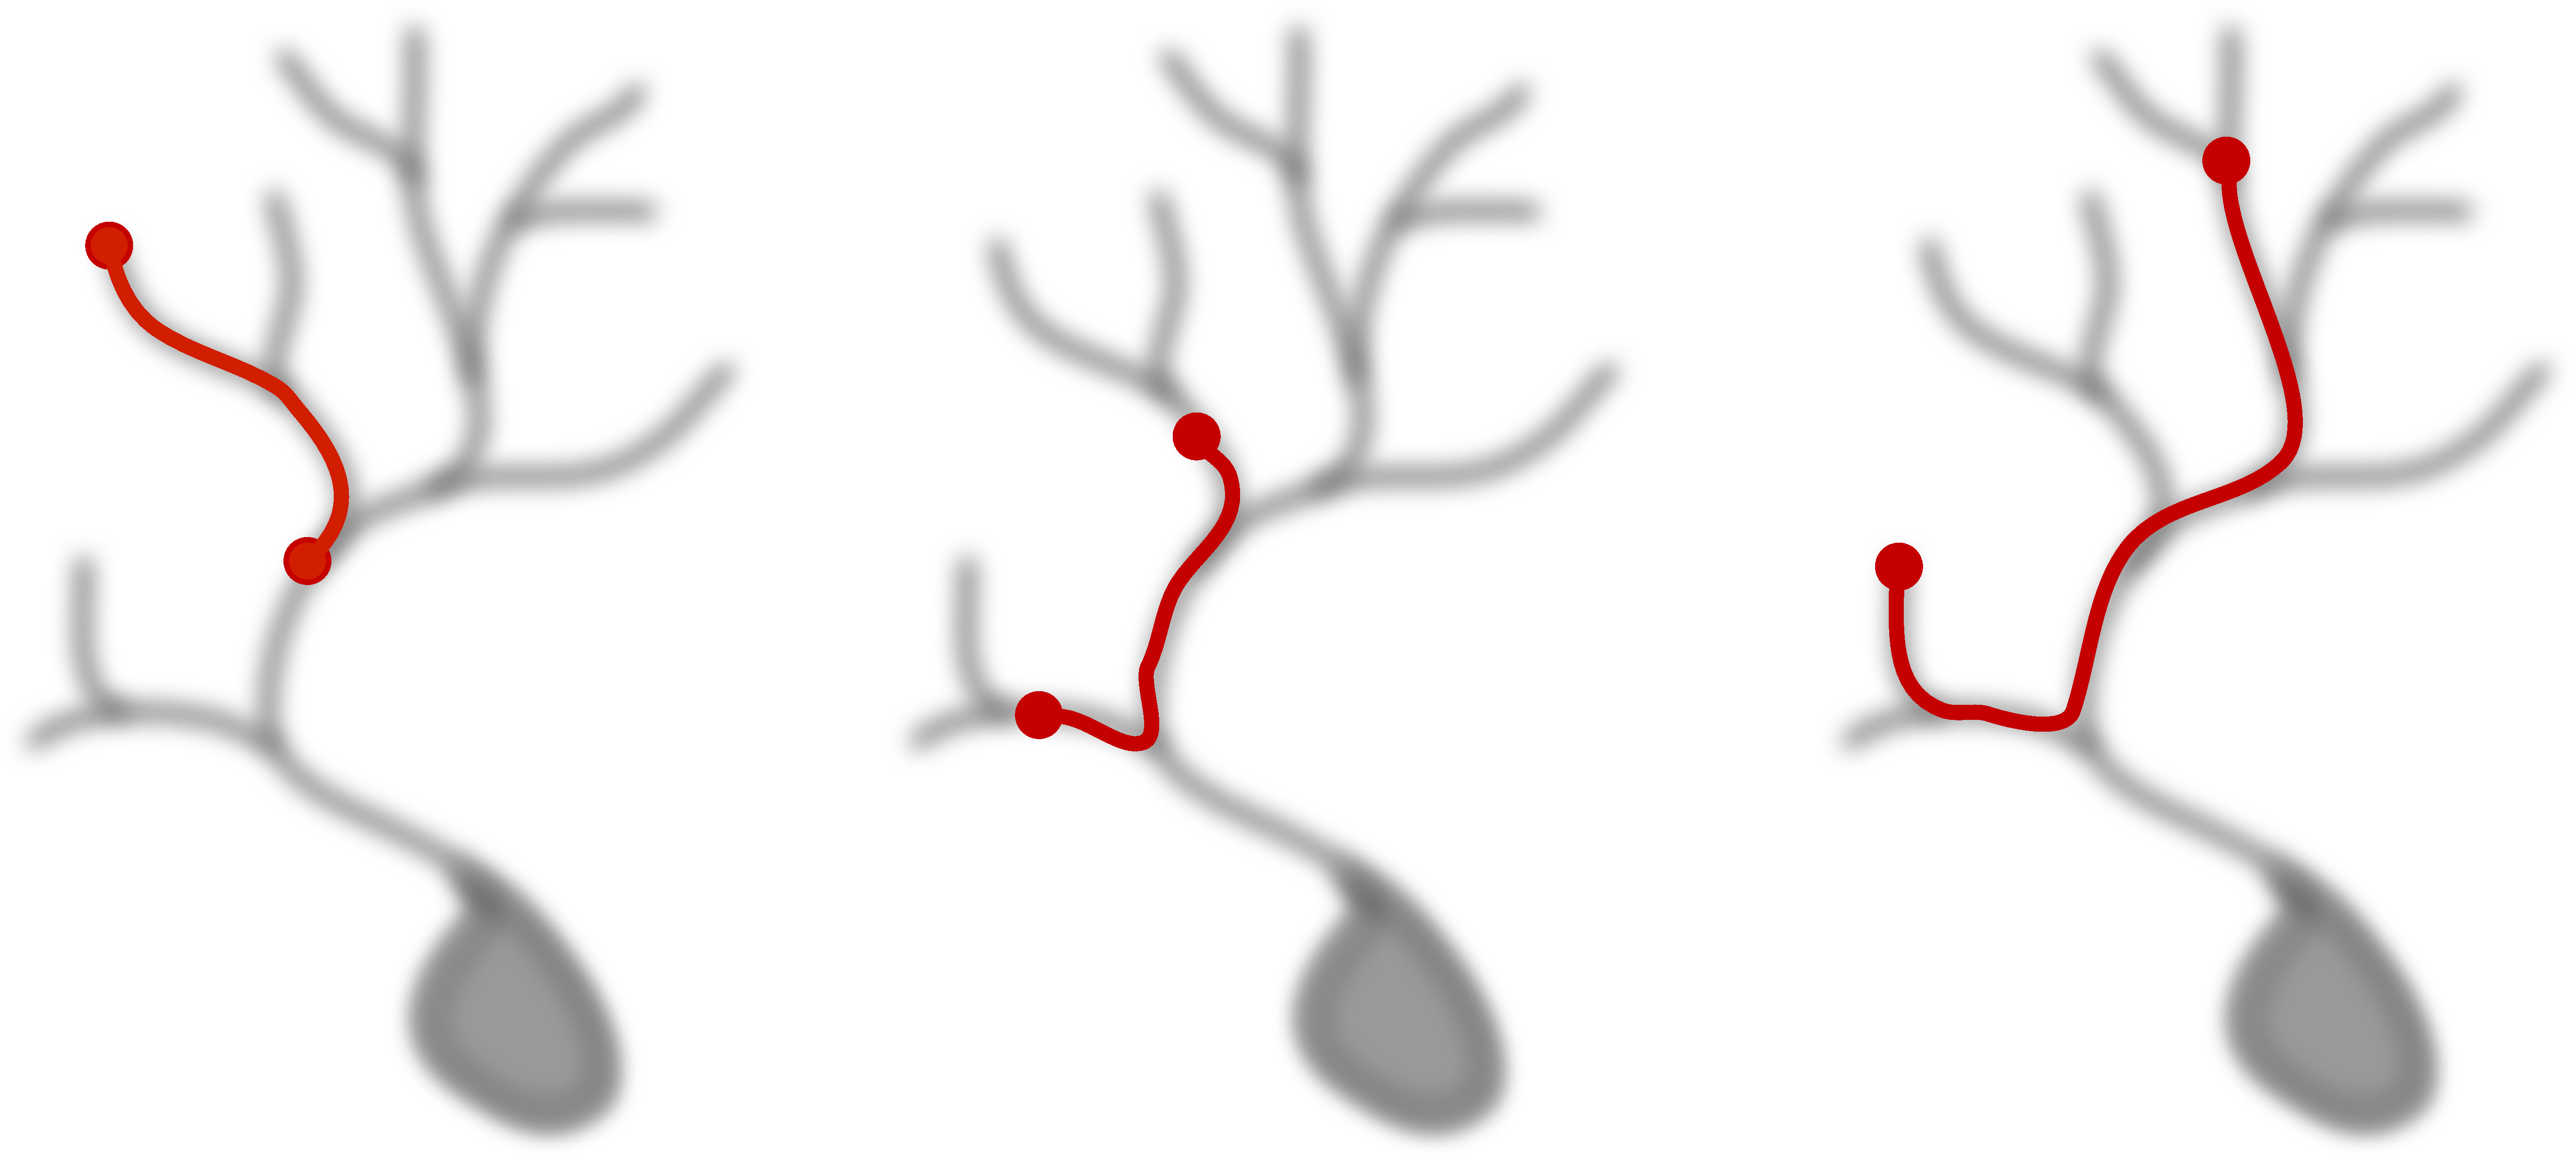
\includegraphics[width=0.5\textwidth]{ch1_fig2}\\
a) Shortest path tracing \\
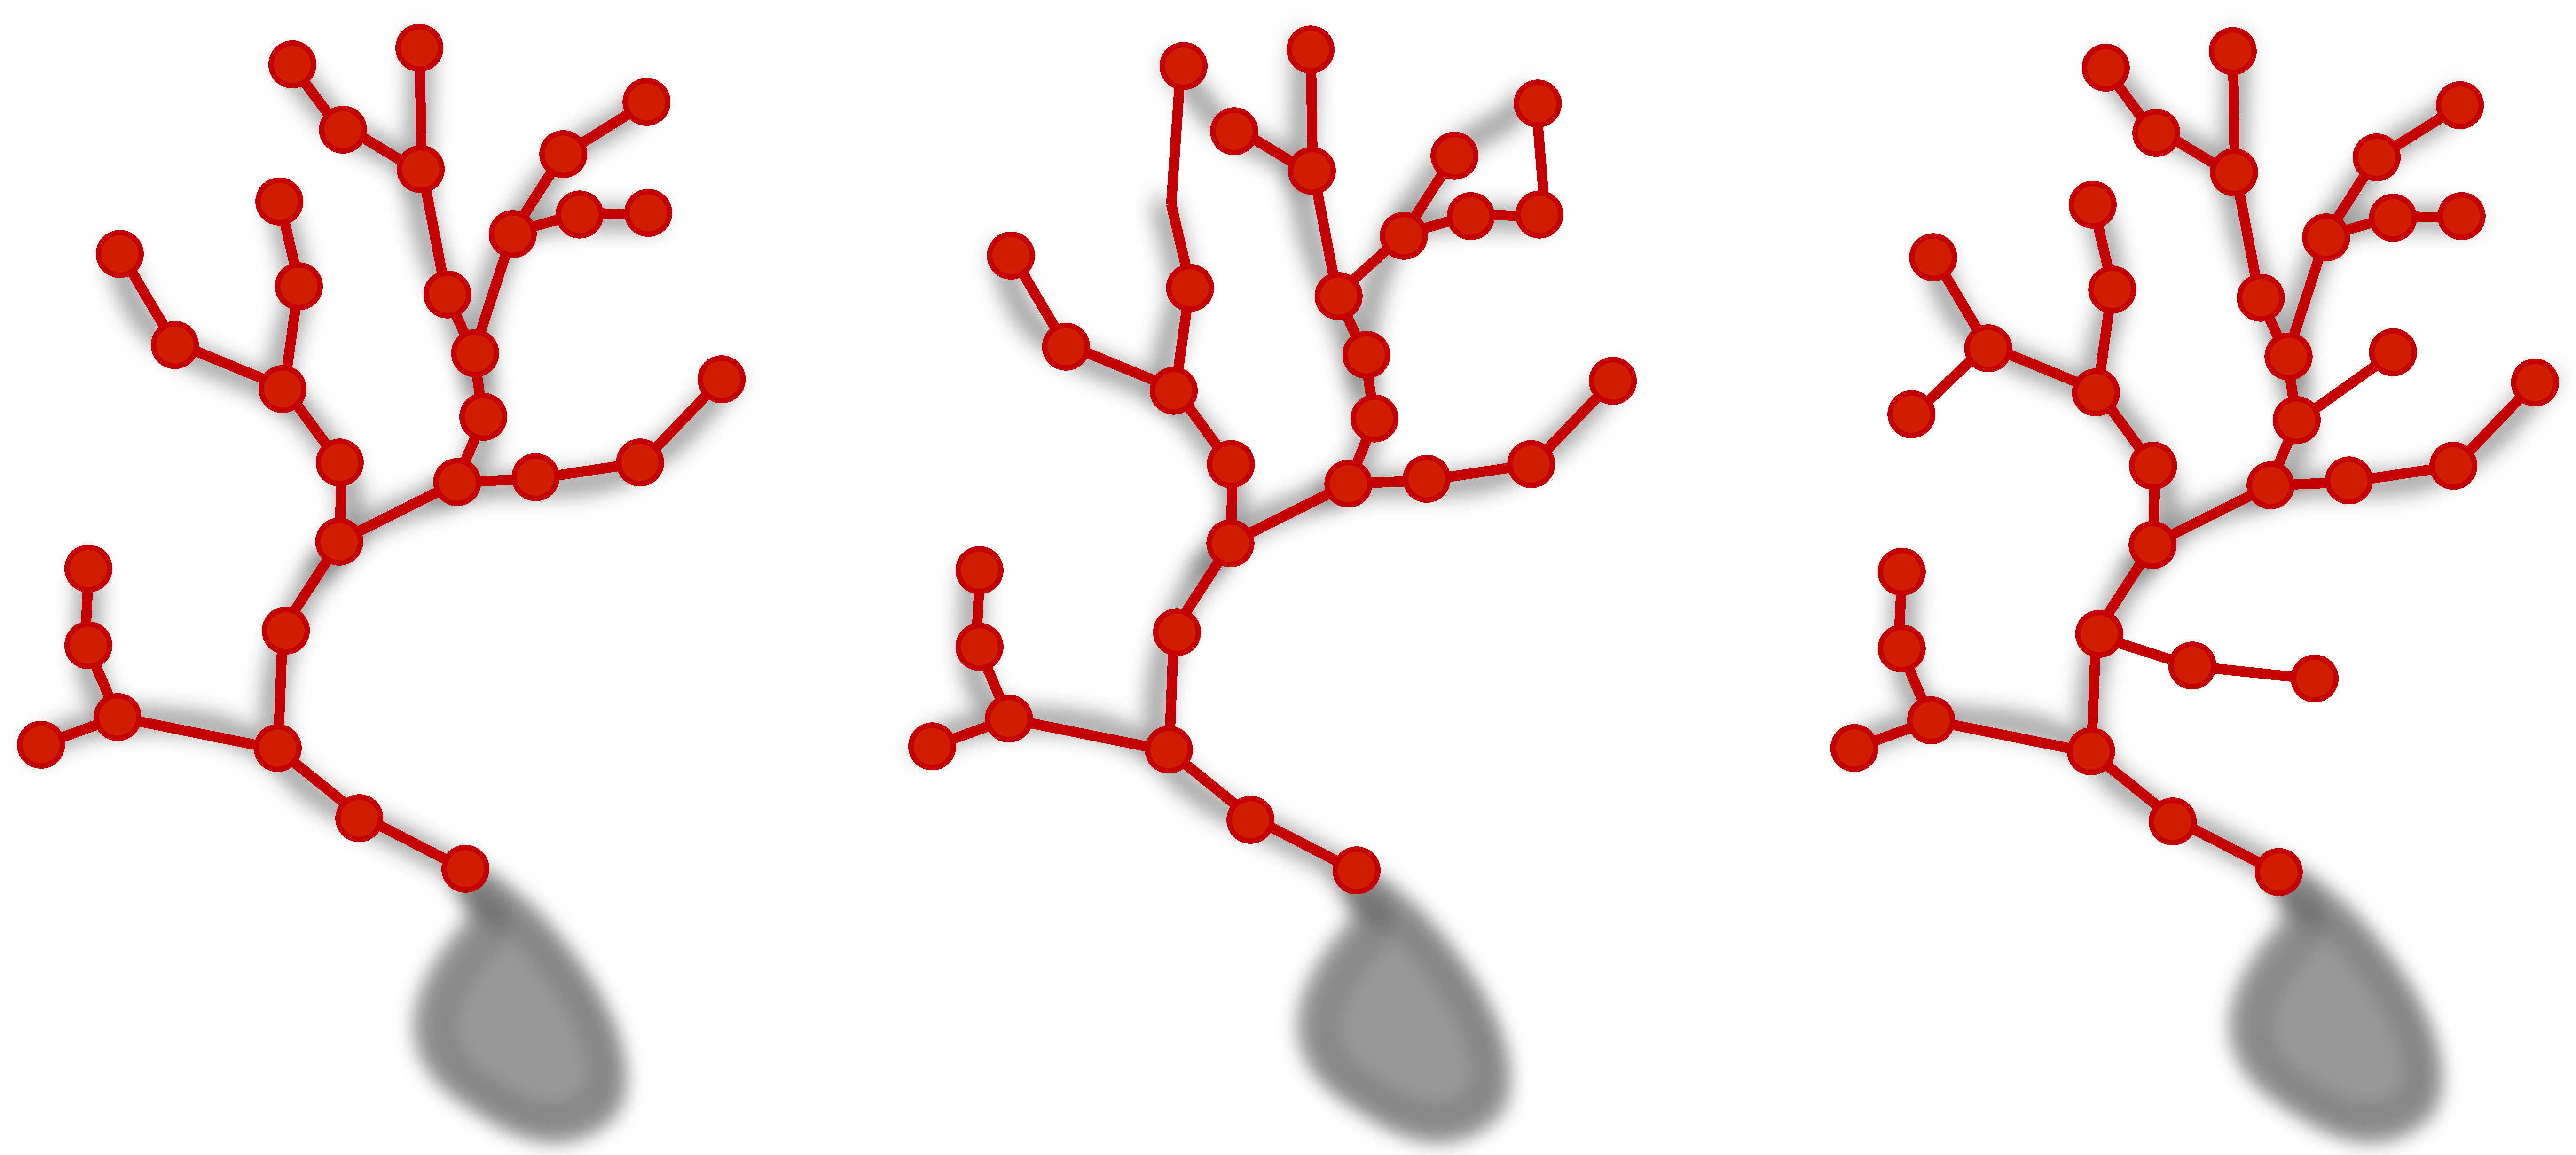
\includegraphics[width=0.5\textwidth]{ch1_fig3}\\
b) Minimum spanning tree \\
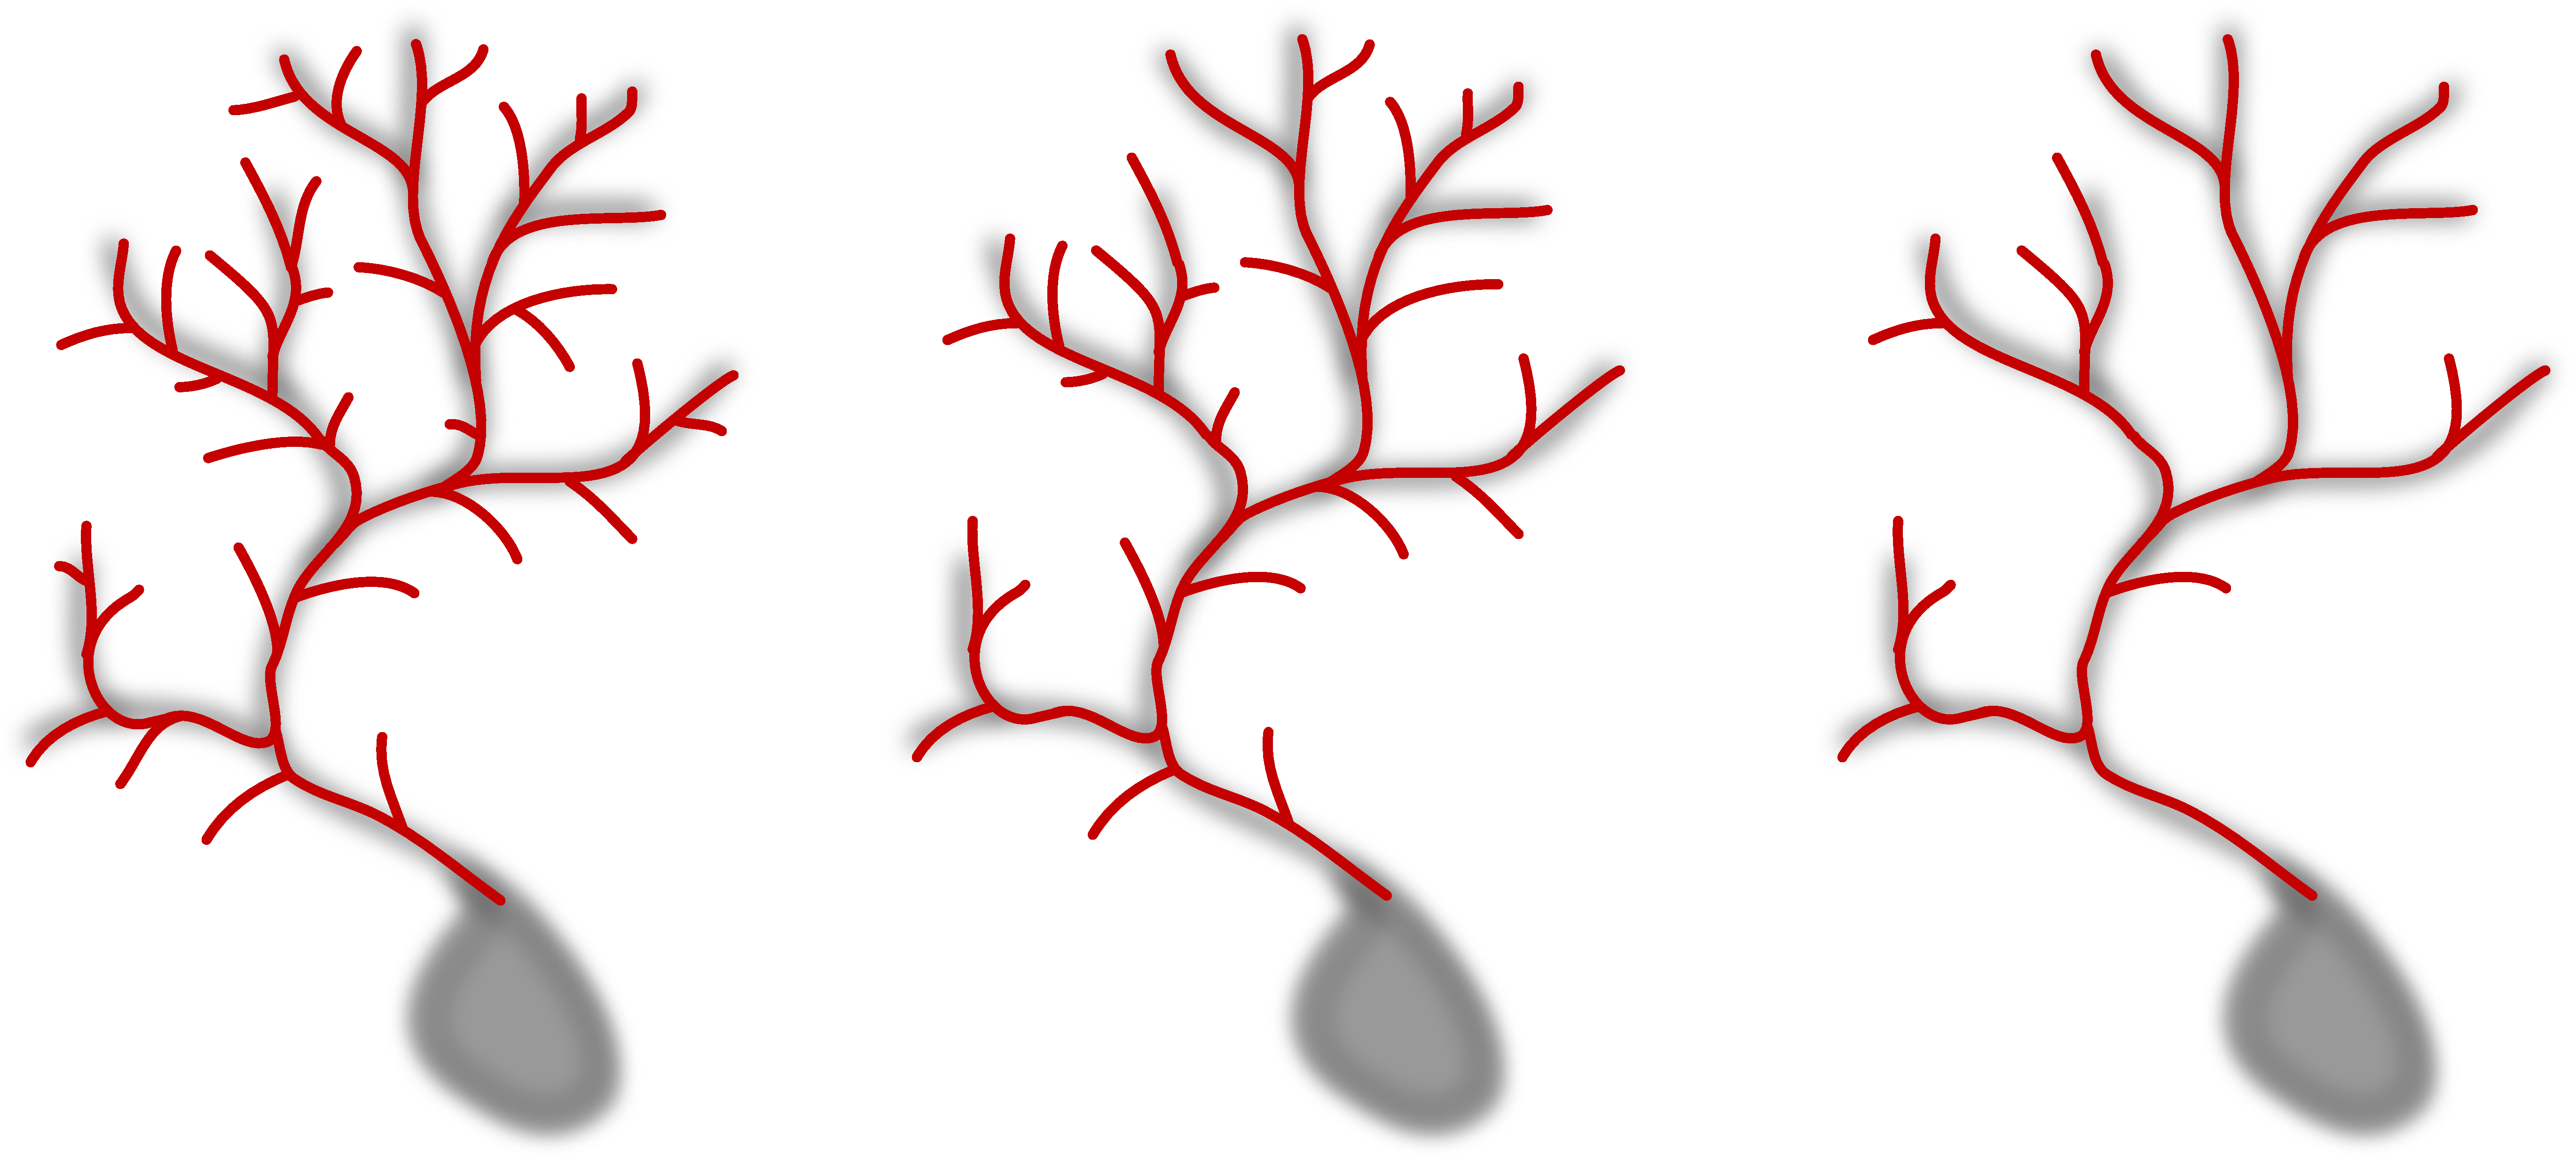
\includegraphics[width=0.5\textwidth]{ch1_fig4}\\
c) Path-prunning
\end{center}
\vspace{-3ex}
\caption{Examples of key neuron reconstruction strategies: a) Finding optimal path between two fixed points, b) Inferring the  optimal tree structure from the given nodes c) Prunning the overcomplete neuron tree.}
\vspace{-1ex}
\label{ch1__fig2-4}
\end{figure}

Computation methods

\section{Examining the neuronal reconstructions}
Once computed, neurons are typically stored in vectorized SWC format. 
\subsection{SWC} 
% source:
% https://www.neuron.yale.edu/phpBB/viewtopic.php?t=3477
%Stockley, E. W.; Cole, H. M.; Brown, A. D. & Wheal, H. V.
%A system for quantitative morphological measurement and electronic modelling of neurons: three-dimensional reconstruction.
%J Neurosci Methods, 1993, 47, 39-51
%
% http://www.neuromorpho.org/myfaq.jsp (What is SWC format?)
% http://research.mssm.edu/cnic/swc.html
% http://www.neuronland.org/NLMorphologyConverter/MorphologyFormats/SWC/Spec.html
The SWC \cite{cannon1998line} is widely used open format for digital neuron reconstruction that describes a reconstruction as a list of 3D nodes (neuronal compartments) with seven attributes (NeuroMorpho.org):  $i$: node index identifier, node type $[0-7]$, node 3D coordinates $(x_i,y_i,z_i)$, radius $(r_i)$ and a parent node index - link towards the predecessor parent node $(j | j=-1)$ if the node has no parent soma node, Fig.~\ref{ch1__fig5}. To define a correct tree structure, each node can only have one predecessor (parent) and the parent node should have lower index so that the indexes of the reconstruction are sorted. Loops and disconnected branches should not exist. The originating node has parend  Etymologically, SWC represents the acronym containing the initials of the last names of Stockley, Wheal, and Cole. Although not directly described in their joint work on quantitative measurement and modeling of the neuron morphology \cite{stockley1993system}, the origin of the SWC name is an acronym of the initials of their last names. Moreover, there is slight uncertainty on the SWC format, especially concerning the unified definition on how soma reconstruction is addressed, so that several variations over the SWC standard can be found\footnote{}.
\begin{figure}
	\begin{center}
		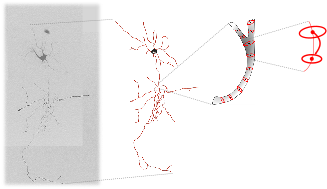
\includegraphics[width=\textwidth]{ch1_fig5} \\
		a 
	\end{center}
	\vspace{-3ex}
	\caption{SWC format of the digital reconstruction. Visualization using Vaa3D \cite{peng2010automatic}}
	\vspace{-1ex}
	\label{ch1__fig5}
\end{figure}

%\begin{figure}[t!]
%	\centering\tiny
%	\begin{tabular}{@{}c@{\hspace{0.02\columnwidth}}c@{\hspace{0.02\columnwidth}}c@{}}
%		& \hspace{3.5em}S = 2 & \hspace{3.5em}S = 3 \\[0.02\columnwidth]
%		\rotatebox{90}{\hspace{0.5em}COR = 0} &
%		\includegraphics[align=c,width=0.47\columnwidth]{synFSnrS2Cor0} & % ./fig/exp.syn/compare_snr/_F(snr,S=2,cor=0)
%		\includegraphics[align=c,width=0.47\columnwidth]{synFSnrS3Cor0} \\ % ./fig/exp.syn/compare_snr/_F(snr,S=3,cor=0)
%		\\[0.01\columnwidth]
%		\rotatebox{90}{\hspace{0.5em}COR = 1} &
%		\includegraphics[align=c,width=0.47\columnwidth]{synFSnrS2Cor1} & % ./fig/exp.syn/compare_snr/_F(snr,S=2,cor=1)
%		\includegraphics[align=c,width=0.47\columnwidth]{synFSnrS3Cor1} % ./fig/exp.syn/compare_snr/_F(snr,S=3,cor=1)
%	\end{tabular}
%	\caption{Average F score of the methods for the synthetic images as a function of SNR. Examples are shown for COR = 0 (top) and 1 (bottom) in combination with S = 2 (left) and 3 (right).}
%	\label{fig:f[snr]_synthetic}
%\end{figure}

\subsection{Measuring distances between neurons}

L-measure, neuro-blast
Distances between neurons can be based on the overlap and the inter-node metric distances.

\section{Thesis outline}
In this thesis probabilistic and bayesian methods are explored.
